\documentclass[a4paper,12pt]{article}
\usepackage[swedish]{babel}
\usepackage[T1]{fontenc}
\usepackage[utf8]{inputenc}
\usepackage{lmodern}
\usepackage{amsmath}
\usepackage{chemformula}
%\usepackage{cite}
\usepackage[parfill]{parskip}
\usepackage[pdftex,
            pdfauthor={Oscar Bohlin},
            pdftitle={Biokemi \--- Samspel mellankKolhydrater och amylas}]{hyperref}
%\usepackage{apacite}
%\usepackage[style=apa,backend=biber]{biblatex}
%\bibliography{källor}
%\bibliography{biblatex-examples}
\hypersetup{pdfborder = {0 0 0}}

\title{Biokemi \--- Samspel mellan kolhydrater och amylas}
\author{Oscar Bohlin}

\begin{document}

\pagenumbering{gobble}
\maketitle
\newpage
\pagenumbering{arabic}
\tableofcontents
\newpage


\section{Introduktion}

\section{Teori}

\subsection{Syfte}

	Syftet med denna laboration är att undersöka kritiska delar i kroppens matspjälkningssystem. Resultaten i denna laboration kan komma att förklara essentiella delar i nedbrytningen av kolhydrater som inte nödvändigvis är koppat till människor, utan andra kommplicerade organismer likaväl. Detta experiment är ett av många för att kunna kartlägga matspjälkningssystemet, dess komponenter och de individuella komponenternas funktion. 

\subsection{Frågeställning}

	\begin{quotation}
		Hur påverkar mängden amylas mängden monomerer som bildas när det utsätts för polymerer.
	\end{quotation}

\subsection{Bakgrundsteori}

\subsubsection{Kolhydrater}

\subsubsection{Enzymer}

	Enzymer är makroproteiner vars syfte är att katalysera reaktioner. En katalysator är en substans eller ett matrial som medverkar i en reaktion utan att förbrukas samt att påskynda reaktionee. Katalysatorer sänker aktiveringsenergin det tar för en reaktion att starta, hur katalysatorer uppnår det beror på fall till fall. 
	
	För att spjälka polymerer till monomerer används bland annat enzymet amylas. Amylas finns främst i salivet i munnen, det spjälker polymererna i födan till monomerer. Däremot utvinner inte amylas någon energi ur polymererna, utan klipper dem endast. Produkten blir monomerer eller reducerat socker, vilket är definerat som enkala sockerarter såsom glukos eller fruktos. De reducerande sockerarterna har förmågan att ingå i oxidations/reduktions reaktioner. 

\subsubsection{Trommers prov}

	Tromemrs prov använder sig av \ch{NaOH} och \ch{CuSO4} så att följaden reaktion sker: 
	\begin{equation}
		\ch{2 NaOH + CuSO4  -> Cu(OH)2 + Na2SO4}
	\end{equation}
	I reaktionen så har kopparsulfatet (\ch{CuSO4}) \textbf{oxiderats/reducerats?} till koppardihydroxid (\ch{Cu(OH)2}), som sedan kan \textbf{oxiderats/reducerats?} med det reducerande sockret i lösningen och produkten blir \ch{Cu+} som har en distikt orangeröd färg jämförelsevis \ch{Cu^2+} eller \ch{CuSO4} som har en distink ljusblå färg. \ch{NaOH} har ingen färg speciell färg, och kan bäst jämföras med vattnets färg. 

	Ju tydligare orangeröd färg desto mer reducerat socker finns i lösningen.

	%\textit{Kopparen har reducerat av reaktionen och kan nu oxidras av det reducerande sockret. \ch{CuSO4} har en tydlig blå färg medan \ch{Cu+} har en brunröd färg. När det oxiderade kopparen kommer i kontakt med det reducerade sockret så får lösningen en orangeröd färg, vilket indikerar att det finns reducerat socker i lösningen.}
	
	



\subsection{Hypotes}

	Eftersom amylas är ett enzym och katalyserar reaktioner, i detta fall polymerer (Stärkelse) $\rightarrow$ monomerer (Reducerat socker) så är det logiskt att tänka att mängden monomerer som bildas ökar linjärt, enlig den generalla formeln $f(x) = k \times x + m$, då x = mängden ammylas och k en okänd konstant. Det är orimligt att $k < 0$ då det skulle innebära att amylas hämmar nedbrytningen av polymerer. Ju mer nedbrytare det finns inom ett kontrollerat område desto mer matrial bryts ned, samma princip i denna laboration. Därför bör det provrör med mest amylas bryta ned mest polymerer.



\section{Metod}

\subsection{Matrial}

\subsubsection{Labbutrustning}

	\begin{itemize}
		\item (1x) Labbrock 						
		\item (1x) Säkerhetsglasögon			
		\item (1x) Värmeplatta 					
		\item (4x) Provrör						
		\item (1x) 100 ml bägare					
		\item (1x) Provrörsställ
	\end{itemize}

\subsubsection{Kemikalier}

	\begin{itemize}
		\item (1x) Kranvattenskälla
		\item (1.75ml) Amylaslösning (saliv)
		\item (2ml) $2.0\frac{g}{mol}$ \ch{NaOh} 
		\item (2ml) $0.1\frac{g}{mol}$ \ch{CuSO4}	
		\item (1.75ml) 1\% stärkelselösning			
	\end{itemize}

\subsection{Utförande}

	\begin{itemize}
		\item En bägare fylldes med 50 ml kranvatten.
		\item Fyra provrör markerades med beteckningarna A,B,C respektive D. 
		\item Samtliga provrör fylldes med $\frac{1}{5}$ 1\% stärkelselösning
		\item Provrör A fylldes med $\frac{1}{4}$ ml amylaslösning. 
		\item Provrör B fylldes med $\frac{1}{2}$ ml amylaslösning. 
		\item Provrör C fylldes med $\frac{1}{1}$ ml amylaslösning. 
		\item Provrör D fylldes inte med någon amylaslösning. 
		\item Amylösningen läts regera i 22 minuter
		\item Bägaren med 100 ml kranvatten placerades på en platta och kokades upp till 100 grader celcius. 
		\item Kemikalierna \ch{NaOH} med koncentrationen $2.0\frac{g}{mol}$ \& \ch{CuSO4} med koncentrationen $0.1\frac{g}{mol}$ ställdes fram med en respektive pipett.
		\item 0.5 ml av respektive kemikalie droppades i samtliga provrör så att innehållet i respektive provrör fick en ljusblå färg.  
		\item Samtliga provrör placerades i den kokande bägaren.
		\item Provrör togs ut ur bägaren efter en färgändring hade skett, vilket indikerade att reaktionen var klar.  
	\end{itemize}


\subsection{Metodmotivering}

	Trommers prov är en variant på Fehlings lösning. Skillnaden mellan Trommers prov och Fehlings lösning är följande: Fehlings lösning innehåller utöver \ch{NaOH} och \ch{CuSO4}, Kaliumnatriumtartrat (\ch{C4H4O6KNa-4H2O}). Detta innebär att resultatet får en större träffsäkerhet. Trots detta valde vi akivt att använda Trommers Prov eftesom den kemikalien inte finns tillänglig till vår befogan. Dessutom skulle den extra träffsäkerheten inte spela någon vidare stor roll eftersom vi undersöker i yttersta grad.  
	
	Vi vade att ha provrör D som "neutral" så det är möjligt att jämföra $\Delta$ koncentrationen av reducerat socker i provrören.


	%Genom följande reaktion \ch{CuSO4 + NaOH} så bildas en klar ljusbå lösning. När denna lösning reagerar med de reducerande sockerarterna från provrören, \ch{stärkelselösning + Amylaslösning -> Glukos}. Det reducerade sockret reagerar med fällningen från följande reaktion och skapar en orange-röd färg. Desto högre koncentration reducerat socker desto mer orange-röd färg. 


\section{Resultat}

\subsection{Utföring 1}

	\begin{figure}[!htb]
		\center{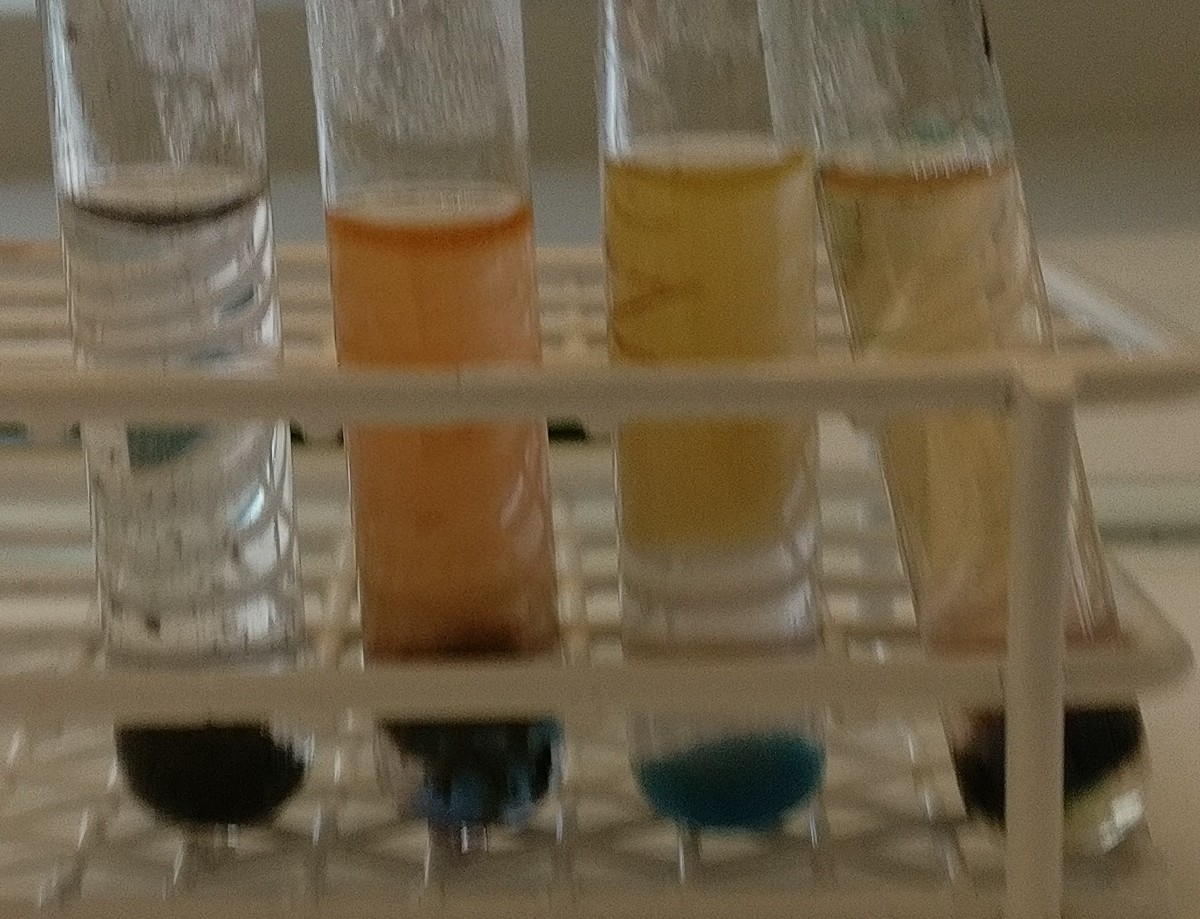
\includegraphics[width=0.7\textwidth]{r1.jpg}}
		\caption{Resultat från första experiment}
		\label{fig:figure_1}
	\end{figure}


\section{Källor}

%\bibliography{mybib}{}
%\bibliographystyle{plain}


%https://sv.wikipedia.org/wiki/Trommers_prov
%https://www.ne.se/uppslagsverk/encyklopedi/l%C3%A5ng/trommers-prov
%Linda
%Kemi/Biologi boken
%sFörelsningar


\end{document}
